\subsection{Model Based Safety Assessment}
\label{subsec:mbsa}

The lack of precise models of the system architecture and its failure modes often forces safety analysts to devote significant effort to gathering architectural details about the system behavior from multiple sources. Furthermore, this investigation typically stops at system level, leaving software function details largely unexplored. Typically equipped with the domain knowledge about the system, but not detailed knowledge of how the software applications are designed, practicing safety engineers find it a time consuming and involved process to acquire the knowledge about the behavior of the software applications hosted in a system and its impact on the overall system behavior. A diagram of this process is shown in Figure~\ref{fig:proposed_safety_process}.

\begin{figure}[h]
	\centering
	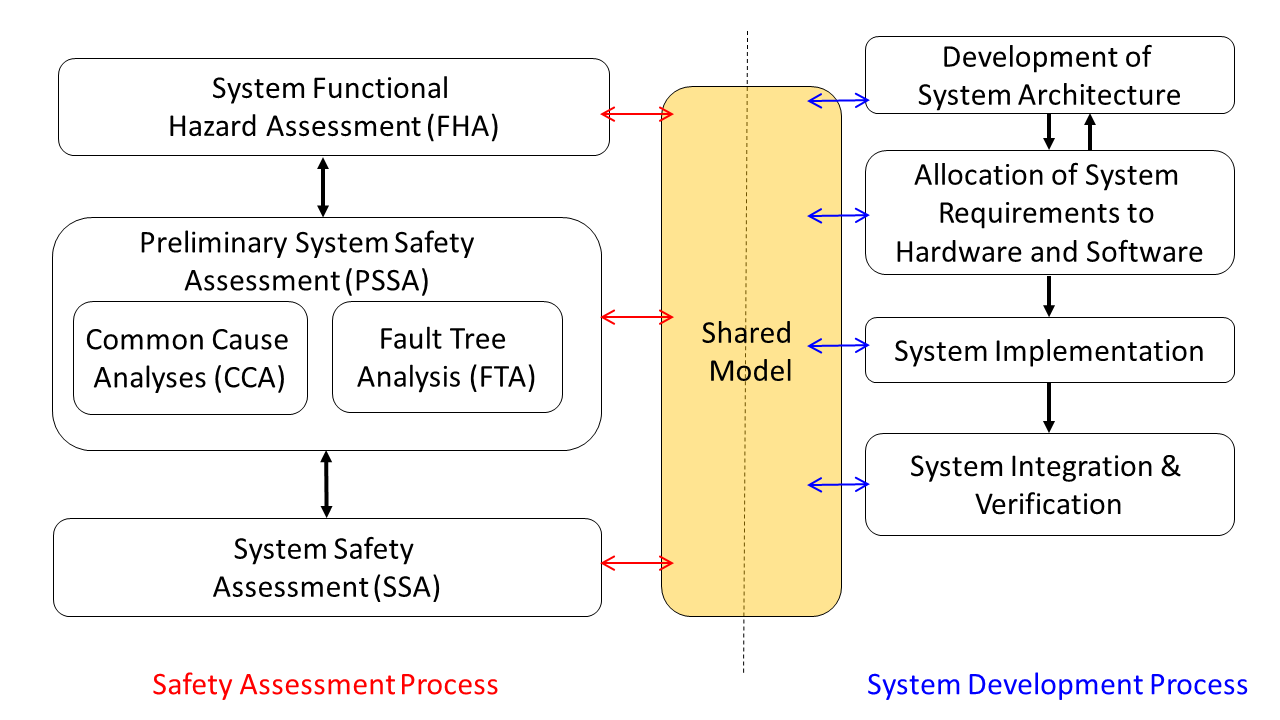
\includegraphics[trim=0 5 0 5,clip,width=0.85\textwidth]{images/process3.png}
	\caption{Use of the Shared System/Safety Model in the ARP4754A Safety Assessment Process}
	\label{fig:proposed_safety_process}
\end{figure}

Industry practitioners have come to realize the benefits of using models in the safety assessment process, and a revision of the ARP4761 to include Model Based Safety Analysis (MBSA) is under way. 

\subsection{Proposed Model Based Safety Assessment Process Supported by Formal Methods}
We propose a model-based safety assessment process backed by formal methods to help safety engineers with early detection of the design issues.  This process uses a single unified model to support both system design and safety analysis; this is shown in Figure~\ref{fig:SACycle1} and is based on the following steps:

\begin{enumerate}
	\item System engineers capture the critical information in a shared model:  high-level hardware and software architecture, nominal behavior at the component level, and safety requirements at the system level.
	\item System engineers use a model checker to check that the safety requirements are satisfied by the nominal design model. 
	\item Safety engineers augment the nominal model with the component failure modes. In addition, safety engineers specify the fault hypothesis for the analysis which corresponds to how many simultaneous faults the system must be able to tolerate.
	\item Safety engineers use a model checker to analyze if the safety requirements and fault tolerance objectives are satisfied by the design in the presence of faults. If the design does not tolerate the specified number of faults (or probability threshold of fault occurrence), then the tool produces counterexamples or minimal sets of fault combinations that can cause the safety requirement to be violated.
	\item The safety engineers examine the results to assess the validity of the fault combinations and the fault tolerance level of the system design. If a design change is warranted, the model will be updated with the latest design change and the above process is repeated.
\end{enumerate}

\begin{figure}[h]
	\begin{center}
		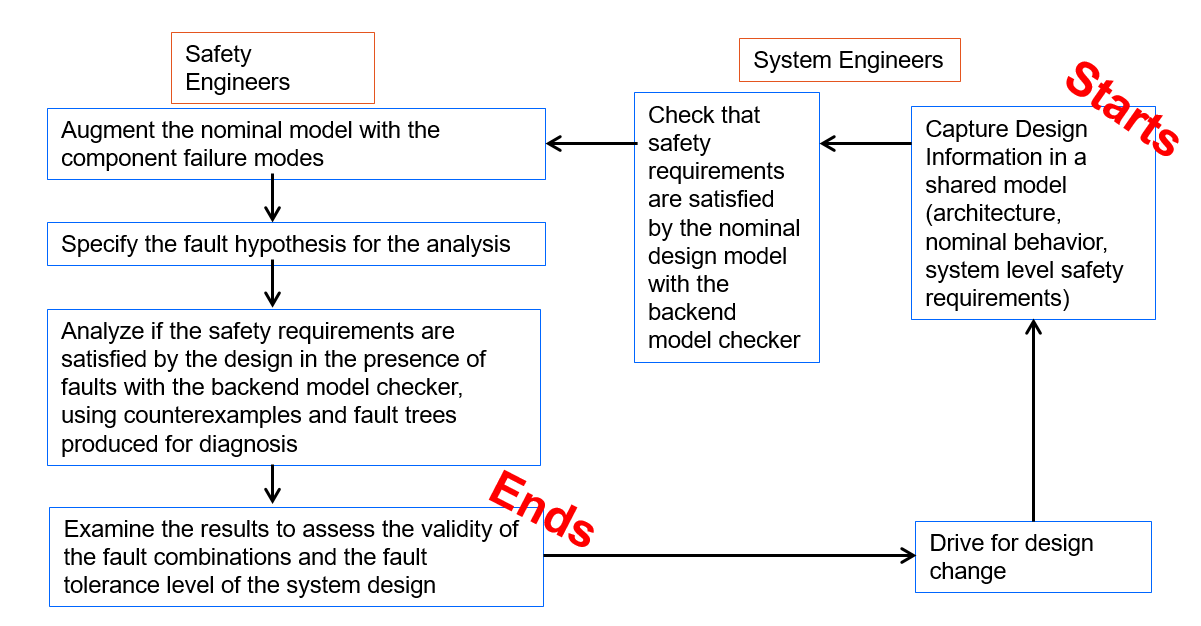
\includegraphics[width=\textwidth]{images/SACycle.PNG}
	\end{center}
	\caption{Proposed Steps of the Safety Assessment Process}
	\label{fig:SACycle1}
\end{figure}

These steps can be viewed as a cyclical process that involves both the system development engineers and the safety engineers of the system. Figure~\ref{fig:SACycle1} shows these steps within the context of the start and end of a project. 

\danielle{Add a bit more information here - pull from the MBSE project for IRAD. Include reasons why this approach is better, how it will help safety analysts, how it benefits the field as a whole. Then lead into the next sections with a statement about model checking, verification, etc.}